\documentclass[usenames,dvipsnames,notes,11pt,aspectratio=169]{beamer}
\usepackage{ifthen}
\usepackage{xcolor}
\usepackage{pgfplots}
\usepackage{amsmath}
\usepackage{centernot}
\usepackage{xspace}
\usepackage{pifont}
\usepackage{tabularx}
\usepackage{makecell}
\usepackage{cuted}
\usepackage{booktabs}
\usepackage{array}
\usepackage{CJKutf8}
\usepackage{textcomp}
\usepackage{setspace}
\usepackage{xparse,mathtools}
\usepackage{pdfcomment}
%\newcommand{\pdfnote}[1]{\marginnote{\pdfcomment[icon=note]{#1}}}
\newcommand{\pdfnote}[1]{}

\usepackage{pgfpages}
%\setbeameroption{show notes on second screen}

\newcommand\w[1]{\textit{#1}}


\input ../beamer-style
\input ../std-macros
\input ../macros

\AtBeginSection[]
{
    \begin{frame}
        \frametitle{Table of Contents}
        \tableofcontents[currentsection]
    \end{frame}
}
\parskip=10pt

\title[CSCI-GA.2590]{Text Classification}
\author[He He]{He He
}
\institute[NYU]{
    
\includegraphics[height=1cm]{../figures/nyu-logo}\\
}
\date{January 24, 2023}

\begin{document}

\begin{frame}
\titlepage
\end{frame}

\begin{frame}
    {Text classification}
    \begin{itemize}
        \item Input: text (sentence, paragraph, document)
        \item Predict the \blue{category or property} of the input text
            \begin{itemize}
                \item Sentiment classification: Is the review positive or negative?
                \item Spam detection: Is the email/message spam or not?
                \item Hate speech detection: Is the tweet/post toxic or not?
                \item Stance classification: Is the opinion liberal or conservative?
            \end{itemize}
            \pause
        \item Predict the \blue{relation} of two pieces of text
            \begin{itemize}
                \item Textual entailment (HW1): does the premise entail the hypothesis?\\
                    Premise: The dogs are running in the park.\\
                    Hypothesis: There are dogs in the park.
                \item Paraphrase detection: are the two sentences paraphrases?\\
                    Sentence 1: The dogs are in the park.\\
                    Sentence 2: There are dogs in the park.
            \end{itemize}
    \end{itemize}
    \pdfnote{
        Paraphrase detection itself may not always be a well-defined problem.
        Consider the given example, are they paraphrase?
        Well, it depends on the context.
        If the task is image caption, then yes.
        If the task is dialogue response generation, where the context is ``Where are the dogs?'',
        then S1 and S2 convey very different answers to the question.
    }
\end{frame}

\section{Generative models: naive Bayes}

\begin{frame}
    {Intuition}
    \begin{itemize}
        \itemsep1em
        \item \textbf{Example}: sentiment classification for movie reviews
    \begin{itemize}
        \item[] {\small \setstretch{0.8} \textit{Action. Comedy. Suspense. This movie has it
all. The Plot goes that 4 would be
professional thieves are invited to take part in a
heist in a small town in Montana. every type of
crime movie archetype character is here. Frank,
the master mind. Carlos, the weapons expert. Max,
the explosives expert. Nick, the safe cracker and
Ray, the car man. Our 4 characters meet up at the train station
and from the beginning none of them like or trust
one another. Added to the mix is the fact that
Frank is gone and they are not sure why they have
called together. Now Frank is being
taken back to New Jersey by the 2 detectives but
soon escapes on foot and tries to make his way
back to the guys who are having all sorts of
            problems of their own. \textcolor<2->{blue}{Truly a great
film loaded with laughs and great acting. Just an
overall good movie for anyone looking for a laugh
            or something a little different}}\par}
    \end{itemize}
    \pause
\item \textbf{Idea}: count the number of positive/negative words
    \begin{itemize}
        \item What is a ``word''?
        \item How do we know which are positive/negative?
    \end{itemize}

    \end{itemize}
    \pdfnote{
        How would you quickly tell the sentiment of this review?
        Understand everything said in it is hard (genre, plot, actor performance etc.).
        But sometimes a couple of keywords or a concluding sentence is sufficient.
    }
    \pdfnote{
        Now there are two questions left.
        We know what's a word intuitively, but to the computer the input is just a string of unicodes, how can we separate that into a list of words.
        The second question is how can we tell which words are positive or negative. The rule based approach is to construct a dictionary of such words, which can be quite effective.
        But here we'll see how to learn this from labeled data.
    }
\end{frame}

\begin{frame}
    {Preprocessing: tokenization}
    \textbf{Goal}: Splitting a string of characters to a sequence of \textbf{tokens} $[x_1, \ldots, x_n]$.

    \textbf{Language-specific solutions}\\
    \begin{itemize}
        \itemsep1em
        \item Regular expression: ``I didn't watch the movie''. $\rightarrow$ [``I'', ``did'', ``n't'', ``watch'', ``the'', ``movie'', ``.''] 
            \begin{itemize}
                \item Special cases: U.S., Ph.D. etc.
            \end{itemize}
        \item Dictionary / sequence labeler: 
            \begin{CJK*}{UTF8}{gbsn}
                ``我没有去看电影。'' $\rightarrow$ [``我'', ``没有'', ``去'', ``看'', ``电影'', ``。'']
            \end{CJK*}
    \end{itemize}

    \pause
    \textbf{General solutions}: don't split by words\\
    \begin{itemize}
        \item Characters:
            [``u'', ``n'', ``a'', ``f'', ``f'', ``a'', ``b'', ``l'', ``e''] 
        \item Subword (\eg byte pair encoding):
            [``un'', ``aff'', ``able\#'']
    \end{itemize}
    \pdfnote{
        Note that for contractions like didn't. We can tokenize it into either did n't or didn 't. Both are okay as long as it's consistent.
        English tokenization gets more complex when there is punctuations or special symbols.
    }
    \pdfnote{Tokenization can have important impact on the performance of downstream learning algorithms.
    }
    \pdfnote{
        Using character sequences (or even byte sequences) we impose mininal prior knowledge on what is a word. Given enough data, the model can probably figure out a reasonable unit of the characters based on their frequencies. But one downside in this approach is that the sequence is now much longer, and the computation time of many algorithms grows with sequence length, which will be expensive for large-scale training.
    }
    \pdfnote{
        A middle ground is to use subword, a unit larger than characters but smaller than words.
        This is commonly used in large-scale models nowadays.
        The BPE algorithms is a simple technique from data compression.
        The basic idea is to recursively merge frequently adjacent symbols into a new symbol (or token).
        The subword found through this algorithm often corresponds to morphemes.
    }
\end{frame}

\begin{frame}
    {Classification: problem formulation}
    \begin{itemize}
        \itemsep1em
        \item \textbf{Input}: a sequence of tokens $x=(x_1, \ldots x_n)$ where $x_i \in \mathcal{V}$.
        \item \textbf{Output}: binary label $y\in \pc{0, 1}$.
        \item \textbf{Probabilistic model}:
            $$
            f(x) = \begin{cases}
 1 & \text{if $p_\theta(y=1\mid x) > 0.5$} \\
 0 & \text{otherwise}
 \end{cases} ,
            $$
            where $p_\theta$ is a distribution parametrized by $\theta\in{\Theta}$.
        \item Modeling question: what's the parametric form of $p_\theta$?
    \end{itemize}
    \pdfnote{
        Choosing $p_\theta$ is the modeling part where our task-specific knowledge comes in: how should the label depend on the text.
    }
\end{frame}

\begin{frame}
    {Modeling $p(y\mid x)$}
    How to write a review:\\
    \pdfnote{A useful starting place for modeling is to gain some intuition on how the task is performed by humans, and then tranform that into mathematical language.}
    \begin{enumerate}
        \item Decide the sentiment by flipping a coin: $p(y)$
        \item Generate word sequentially conditioned on the sentiment  $p(x\mid y)$
    \end{enumerate}
    \pause
    \vspace{-1ex}
    \onslide<+->{
        \begin{align}
            p(y)&=\onslide<+->{\text{Bernoulli}(\alpha)} \\
            p(x\mid y)&=\onslide<+->{\prod_{i=1}^n p(x_i\mid y)\quad\quad \text{(independent assumption)}}\\
                &=\onslide<+->{\prod_{i=1}^n \text{Categorical}(
                \underbrace{\theta_{1,y},\ldots,\theta_{|\sV|,y}}_{\text{sum to 1}}
                )}
        \end{align}
    }
    \vspace{-1ex}
    \onslide<+->{
        \textbf{Bayes rule}: 
        $$
        p(y\mid x) = \frac{p(x\mid y)p(y)}{p(x)}
        = \frac{p(x\mid y)p(y)}{\sum_{y\in\mathcal{Y}} p(x\mid y)p(y)}
        $$
}
\end{frame}

\begin{frame}
    {Naive Bayes models}
    \begin{block}
    {Naive Bayes assumption}
        The input features are \textbf{conditionally independent} given the label:
        $$
        p(x\mid y) = \prod_{i=1}^n p(x_i\mid y) \;.
        $$
    \end{block}
    \begin{itemize}
        \item A strong assumption, but works surprisingly well in practice.

        \item Note: $p(x_i\mid y)$ doesn't have to be a categorical distribution (\eg Gaussian distribution)
    \end{itemize}

\end{frame}

\begin{frame}
    {Learning: maximum likelihood estimation}
    \textbf{Task}: estimate parameters $\theta$ of a distribution $p(y; \theta)$ given i.i.d. samples $D=\p{y_1, \ldots, y_N}$ from the distribution.

    \textbf{Goal}: find the parameters that make the observed data most probable.

    \pause
    \textbf{Likelihood function} of $\theta$ given $D$:
    $$
    L(\theta; D) \eqdef p(D;\theta) = \prod_{i=1}^N p(y_i; \theta) \;.
    $$

    \textbf{Maximum (log-)likelihood estimator}:
    \begin{align}
        \hat{\theta} &= \argmax_{\theta\in\Theta} L(\theta; D)
        = \argmax_{\theta\in\Theta} \sum_{i=1}^N \log p(y_i; \theta)
    \end{align}

    \pdfnote{To make ``most probable'' more precise, we define the likelihood function of the parameters to be the probability of the data given by the model.}
    \pdfnote{Why can we write the joint distribution as the product? Independent assumption from iid.}
    \pdfnote{Now it's reduced to an optimization problem.}
\end{frame}

\begin{frame}
    {MLE and ERM}
    ERM:
    $$
    \min \sum_{i=1}^N \ell(x^{(i)}, y^{(i)}, \theta)
    $$
    \pause

    MLE:
    $$
    \max \sum_{i=1}^N \log p(y^{(i)} \mid x^{(i)}; \theta)
    $$
    \pause

    What's the connection between MLE and ERM?

    MLE is equivalent to ERM with the \textbf{negative log-likelihood} (NLL) loss function:
    $$
    \ell_{\text{NLL}}(x^{(i)}, y^{(i)}, \theta) \eqdef -\log p(y^{(i)} \mid x^{(i)}; \theta)
    $$
\end{frame}

%\begin{frame}
%    {MLE for our Naive Bayes model}
%    {[board]}
%\end{frame}

\begin{frame}
    {MLE solution for our Naive Bayes model}
    \begin{align*}
        \text{count}(w, y) &\eqdef \text{frequency of $w$ in documents with label $y$}\\[1em]
        p_{\text{MLE}}(w\mid y) &= \frac{\text{count}(w, y)}{\sum_{w\in\mathcal{V}}\text{count}(w, y)}\\
        &= \text{how often the word occur in positive/negative documents}\\
        &= \text{``positive/negative score of the word''}\\[1em]
        p_{\text{MLE}}(y=k) &= \frac{\sum_{i=1}^N \1\p{y^{(i)}=k}}{N}\\
        &= \text{fraction of positive/negative documents}
    \end{align*}

    %\textbf{Smoothing}: reserve probability mass for unseen words
    %$$
    %    p(w\mid y) = \frac{{\color{blue}\alpha} + \text{count}(w, y)}{\sum_{w\in\mathcal{V}}\text{count}(w, y) + {\color{blue}\alpha|\mathcal{V}|}}
    %$$
    %Laplace smoothing: $\alpha=1$
    %\pdfnote{
    %    How well would this model generalize to unseen documents?
    %    What if we have a word that's not seen during training?
    %}
\end{frame}

\begin{frame}
    {Inference: make predictions using the model}

    \textbf{Inference}: $y=\argmax_{y\in\sY} p_\theta(y\mid x)$ 

    \pause
    Compare $p_\theta(y=1\mid x)$ and $p_\theta(y=0\mid x)$:
    \begin{align*}
        \frac{p_\theta(y=1\mid x)}{p_\theta(y=0\mid x)} = 
        \frac{p_\theta(x\mid y=1)p_\theta(y=1)}{p_\theta(x\mid y=0)p_\theta(y=0)}
    \end{align*}

    \pause
    Assuming $p_\theta(y=1)=p_\theta(y=0)$, we only need to compare $p_\theta(x\mid y=1)$ and $p_\theta(x\mid y=0)$.
    \begin{align*}
        \text{score of class $k$} = \log p_\theta(x \mid y=k) = \sum_{i=1}^n \log p_\theta(x_i \mid y=k) 
    \end{align*}
    (Adding up positive/negative scores of each word)
\end{frame}

\begin{frame}
    {Feature design}
        Naive Bayes doesn't have to use single words as features
    \begin{itemize}
        \itemsep1em
        \item Lexicons, \eg LIWC.
        \item Task-specific features, \eg is the email subject all caps.
        \item Bytes and characters, \eg used in language ID detection.
        %\item $n$-grams (a symbol of $n$ consecutive tokens)
    \end{itemize}
    \pdfnote{
        Char/byte NB model is a very fast and effective language ID detector (e.g., google translate).
    }
\end{frame}

\begin{frame}
    {Summary of Naive Bayes models}
    \begin{itemize}
        \item Modeling: the conditional indepedence assumption simplifies the problem
        \item Learning: MLE (or ERM with negative log-likelihood loss)
        \item Inference: very fast (adding up scores of each word)
    \end{itemize}
\end{frame}

\section{Discriminative models: logistic regression}

\begin{frame}
    {Discriminative models}
    % TODO: move this slides to later
    \textbf{Idea}: directly model the conditional distribution $p(y\mid x)$
    \pause
    \begin{table}
        \renewcommand{\arraystretch}{1.5}
        \begin{tabular}{lcc}
            & generative models & discriminative models \\
            \hline
            modeling & joint: $p(x,y)$ & conditional: $p(y\mid x)$ \\
            assumption on $y$ & yes & yes \\
            assumption on $x$ & yes & no \\
            development & generative story & feature extractor
        \end{tabular}
    \end{table}
    \pdfnote{
        In Naive Bayes model, we used Bayes rule to get $p(y\mid x)$ given $p(x\mid y)$ and the class prior $p(y)$.
        But one question here is, if $p(y\mid x)$ is what we are ultimately interested in, why bother modeling the data likelihood and the prior as opposed to directly modeling $p(y\mid x)$.
    }
\end{frame}

\begin{frame}
    {Model $p(y\mid x)$}
    How to model $p(y\mid x)$?
    \begin{itemize}
        \item[] $y$ is a Bernoulli variable:
            $$
            p(y\mid x) = \alpha^y (1-\alpha)^{(1-y)}
            $$
            \pause
        \item[] Bring in $x$:
            $$
            p(y\mid x) = h(x)^y (1-h(x))^{(1-y)} \quad h(x) \in [0,1]
            $$
    \end{itemize}

    \pause
    Parametrize $h(x)$ using a linear function:\\
    $$
    h(x) = w\cdot \phi(x) + b \quad\quad \phi\colon \sX \rightarrow \BR^d
    $$

    Problem: $h(x) \in \BR$ (score)
\end{frame}

\begin{frame}
    {Logistic regression}
    Map $w\cdot\phi(x) \in\mathbb{R}$ to a probability by the \textbf{logistic function}
    \vspace{-1em}
    \begin{center}
        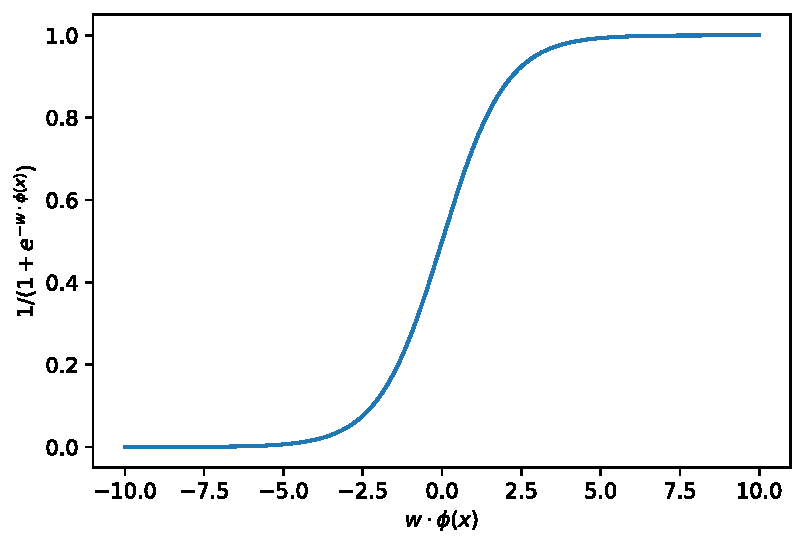
\includegraphics[height=4cm]{figures/logistic}
    \end{center}
    \vspace{-2em}
    \begin{align*}
    p(y=1\mid x; w) &= \frac{1}{1 + e^{-w\cdot\phi(x)}} \quad (y\in \pc{0,1})\\\pause
        p(y=k\mid x; w) &= \frac{e^{w_k\cdot\phi(x)}}{\sum_{i\in\mathcal{Y}}e^{w_i\cdot\phi(x)}} \quad (y\in \pc{1, \ldots, K}) && \text{``softmax''}
    \end{align*}
    \pdfnote{
        Note that in multiclass classification setting, there is one $w$ for each class.
    }
\end{frame}

\begin{frame}
    {Inference}
    \begin{align}
        \hat{y} &= \argmax_{k\in\sY} p(y=k\mid x; w) \\
        &= \argmax_{k\in\sY} \frac{e^{w_k\cdot\phi(x)}}{\sum_{i\in\mathcal{Y}}e^{w_i\cdot\phi(x)}} \\
        &= \argmax_{k\in\sY} e^{w_k\cdot\phi(x)} \\
        &= \argmax_{k\in\sY} \underbrace{w_k\cdot\phi(x)}_{\textstyle\text{score for class $k$}}
    \end{align}
\end{frame}

\begin{frame}
    {MLE for logistic regression}
    \begin{itemize}
        \item Likelihood function is concave / NLL is convex
        \item No closed-form solution 
        \item Use stochastic gradient ascent 
    \end{itemize}
    \pdfnote{LR is probabilisti, so we can still do MLE.}
\end{frame}

\begin{frame}
    {BoW representation}
    Example:
    \begin{align*}
        \mathcal{V} &= \pc{\w{the}, \w{a}, \w{an}, \w{in}, \w{for}, \w{penny}, \w{pound}}\\
        \text{sentence} &= \w{in for a penny, in for a pound} \\
        x &= \p{\w{in}, \w{for}, \w{a}, \w{penny}, \w{in}, \w{for}, \w{a}, \w{pound}}
    \end{align*}

    \textbf{Feature extractor}: $\phi\colon \mathcal{V}^n \rightarrow \mathbb{R}^d$.
    \pause

    \textbf{Idea}: a sentence is the ``sum'' of words.
    $$
    \phi_{\text{BoW}}(x) = \sum_{i=1}^n \phi_{\text{one-hot}}(x_i)
    $$
    \vspace{-1em}

    \begin{align*}
        \phi_{\text{one-hot}}(x_1) &= \begin{bmatrix} 0 & 0 & 0 & 1 & 0 & 0 & 0 \end{bmatrix}
        \quad \text{the sentence contains the word ``in''}\\
        \phi_{\text{BoW}}(x)  &= \begin{bmatrix} 0 & 2 & 0 & 2 & 2 & 1 & 1 \end{bmatrix}
        \quad \text{the sentence contains 2 occurrences of ``in''}\\
    \end{align*}
\end{frame}

%\begin{frame}
%    {Compare with naive Bayes}
%    \begin{itemize}
%        \itemsep2em
%        \item Our naive Bayes model ($x_i \in \pc{1, \ldots, |\sV|}$):
%            $$
%            X_i \mid Y=y \sim \text{Categorical}(\theta_{1,y}, \ldots, \theta_{|\sV|, y}) \;.
%            $$
%        \item The naive Bayes generative story produces a BoW vector following a multinomial distribution:
%            $$
%            \phi_{\text{BoW}}(X) \mid Y=y \sim \text{Multinomial}(\theta_{1,y}, \ldots, \theta_{|\sV|,y}, n) \;.
%            $$
%
%        \pause
%        \item Both multinomial naive Bayes and logistic regression learn a linear separator $w\cdot\phi_{\text{BoW}}(x)+b=0$.
%    \end{itemize}
%    \pause
%    Question: what's the advantage of using logistic regression?
%
%    \pdfnote{
%        In this sense, NB is trying to model the BoW feature vector.
%    }
%    \pdfnote{
%        In addition, they both learn a linear predictor which simply sums the score of each word at inference time.
%        For NB, $w$ is $\log \theta$.
%    }
%\end{frame}

%\begin{frame}
%    {Feature vectors for multiclass classification}
%    Multinomial logistic regression
%    \begin{tikzpicture}
%        \node (a) {
%            \begin{minipage}{\textwidth}
%            \begin{align*}
%        p(y=k\mid x; w) =
%             \frac{e^{{\color{blue}w_k\cdot\phi(x)}}}
%                {\sum_{i\in\mathcal{Y}}e^{w_i\cdot\phi(x)}} \quad (y\in \pc{1, \ldots, K})
%            \end{align*}
%            \end{minipage}
%};
%        \node(b) [below= of a] {
%            \begin{minipage}{\textwidth}
%    $$
%        p(y=k\mid x; w) =
%                \frac{e^{{\color{blue}w\cdot\Psi(x, k)}}}{\sum_{i\in\mathcal{Y}}e^{w\cdot\Psi(x, i)}} \quad (y\in \pc{1, \ldots, K})
%    $$
%            \end{minipage}
%};
%        \draw[arrow] (a) -- (b);
%    \end{tikzpicture}
%    scores of each class $\rightarrow$ compatibility of an input and a label
%
%    \pause
%    Multivector construction of $\Psi(x,y)$:
%    $$
%    \Psi(x, 1) \eqdef \pb{\underbrace{0}_{\textstyle y=0}, \underbrace{\phi(x)}_{\textstyle y=1}, \ldots, \underbrace{0}_{\textstyle y=K}}
%    $$
%\end{frame}

\begin{frame}
    {N-gram features}
    Potential problems with the the BoW representation?

    \pause
    \textbf{N-gram} features:
    \begin{center}
        \textit{in for a penny , in for a pound}
    \end{center}
    \begin{itemize}
        \item Unigram: in, for, a, ...
        \item Bigram: in/for, for/a, a/penny, ...
        \item Trigram: in/for/a, for/a/penny, ...
    \end{itemize}

    \think{What are the pros/cons of using higher order n-grams?}
    \pdfnote{
        BoW problem: new york, don't like
    }
\end{frame}

\begin{frame}
    {Feature extractor}
    Logistic regression allows for richer features (what's the limitation of NB?)

    Define each feature as a function $\phi_i\colon \mathcal{X} \rightarrow \BR$.
    \begin{align*}
 \phi_1(x) &= \begin{cases}
 1 & \text{$x$ contains ``happy''} \\
 0 & \text{otherwise}
 \end{cases} ,
 \\
 \phi_2(x) &= \begin{cases}
 1 & \text{$x$ contains words with suffix ``yyyy''} \\
 0 & \text{otherwise}
 \end{cases} .
    \end{align*}
    In practice, use a dictionary
    $$
    \texttt{feature\_vector}[\texttt{"prefix=un+suffix=ing"}] = 1
    $$
    \pdfnote{
        With NB, we can still include these features as variables, but we'll have to think about modeling them as a parametrized distribution and handling the sparsity problem during estimation.
    }
\end{frame}


\section{Regularization, model selection, evaluation}

\begin{frame}
    {Error decomposition}
    Let's ignore the optimization error, assuming we always find the optimum
$$
        \text{risk}(\hat{h}) - \text{risk}(h^*) = \text{approximation error} + \text{estimation error}
        $$
        \vspace{-3em}
    \begin{itemize}
        \itemsep1em
        \item Approximation error:
            $\text{risk}(\text{best hypo in $\sH$}) - \text{risk}(h^*)$ \\
            Does my hypothesis space contain the true hypothesis?
        \item Estimation error:
            $\text{risk}(\hat{h}) - \text{risk}(\text{best hypo in $\sH$})$ \\
            Can I find the best hypothesis given limited data?
    \end{itemize}

    \pause
    Larger hypothesis class: approximation error $\downarrow$, estimation error $\uparrow$

    Smaller hypothesis class: approximation error $\uparrow$, estimation error $\downarrow$

    How to control the size of the hypothesis class?
\end{frame}

\begin{frame}
    {Reduce the dimensionality}
    Linear predictors: $\sH = \pc{w : w \in \BR^d}$

    Reduce the number of features. (Ideas for text classification?)
    \pdfnote{
        stopwords, stemming, filter by frequency
    }
    \pdfnote{
        feature selection (fwd/bwd), L1
    }

    \pause
    For other predictors:\\
    \begin{itemize}
        \item Depth of decision trees
        \item Degree of polynomials
        \item Number of decision stumps in boosting
    \end{itemize}
\end{frame}

\begin{frame}
    {Regularization}
    Reduce the ``size'' of $w$:
    $$
    \min_w \underbrace{\frac{1}{N}\sum_{i=1}^N L(x^{(i)}, y^{(i)}, w)}_{\textstyle \text{average loss}}
    + \underbrace{\frac{\lambda}{2}\|w\|_2^2}_{\textstyle \ell_2 \text{ norm}}
    $$

    Why is small norm good? Small change in the input doesn't cause large change in the output.

\end{frame}

\begin{frame}
    {Gradient descent with $\ell_2$ regularization}
    Run SGD on 
    $$
    \min_w \underbrace{\frac{1}{N}\sum_{i=1}^N L(x^{(i)}, y^{(i)}, w)}_{\text{average loss}}
    + \underbrace{\frac{\lambda}{2}\|w\|_2^2}_{\ell_2 \text{ norm}}
    $$

    Also called \textbf{weight decay} in the deep learning literature:
    $$
    w \leftarrow w - \eta(\nabla_w L(x, y, w) + {\color{blue}\lambda w})
    $$

    Shrink $w$ in each update.
\end{frame}

\begin{frame}
    {Hyperparameter tuning}
    \textbf{Hyperparameters}: parameters of the learning algorithm (not the model)

    Example: use MLE to learn a logistic regression model using BoW features \\
    \bigskip
    \pause

    \pause
    How do we select hyperparameters?\\
    \begin{itemize}
        \item[] Pick those minimizing the training error?
        \item[] Pick those minimizing the test error?
    \end{itemize}
    \pdfnote{What are the hyperparams in this case?}
    \pdfnote{
        Dillema: training error overfit. test error don't know.
    }
\end{frame}

\begin{frame}
    {Validation}
    \textbf{Validation set}: a subset of the training data reserved for tuning the learning algorithm (also called the \textbf{development set}).

    \textbf{$K$-fold cross validation}\\
    {[board]}

    \pause
    It's important to look at the data and errors during development, but \textcolor{red}{not the test set}.
\end{frame}

\end{document}
